%%% Appendix including ripple stuf %%%

\chapter{Open-loop ripple simulations} \label{app:OL_ripple}
The figures in this chapter shows the waveforms of the current and voltage ripples under worst case conditions. These conditions have been described during the calculations of the passive components in section \ref{component_sizing}. The maximum, minimum and mean values will be read and used to calculated the ripples in section \ref{opsimresult}. The data from the simulations have been loaded into Matlab to achieve accurate readings.

Figure \ref{fig:inductor_ripple} shows the current ripple in the inductor. The maximum and minimum currents are read as $I_{max} = 3.465A$ and $I_{min} = 3.135A$, with a mean at $\widebar{I_L} = 3.3A$.


\begin{figure}[H]
	\begin{minipage}[c]{0.5\textwidth}
		\centering
		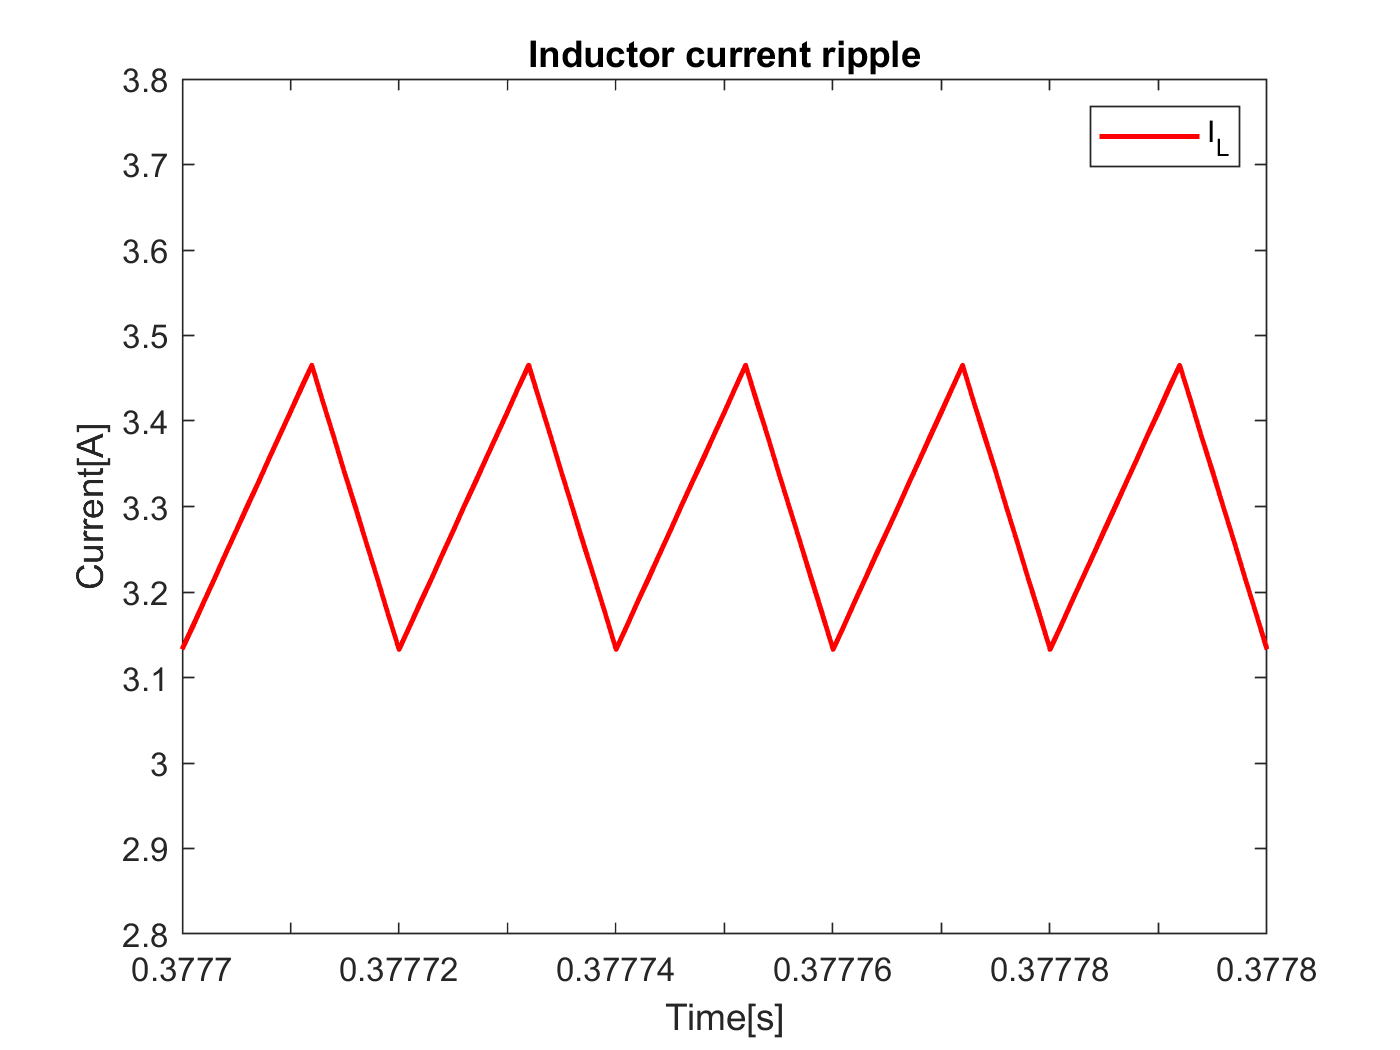
\includegraphics[width=1\textwidth]{../Pictures/P1/Open_loop_simulation/open_loop_IL_ripple} % Left picture
		\caption{Inductor current ripple.}
		\label{fig:inductor_ripple}
	\end{minipage}
	\hfill
	\begin{minipage}[c]{0.5\textwidth}
		\centering
		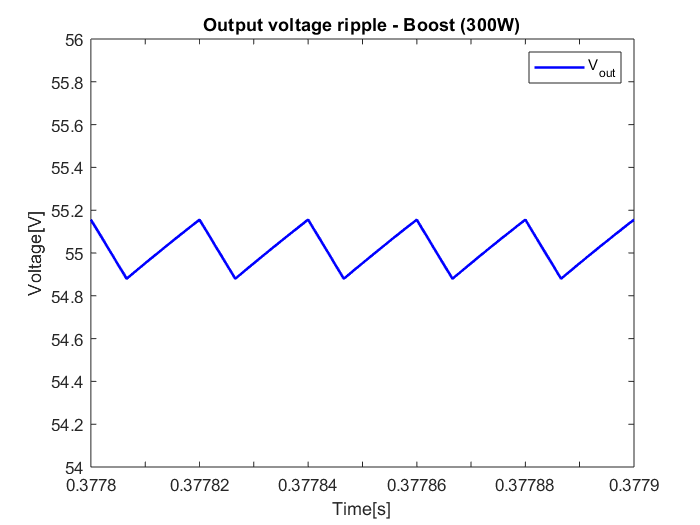
\includegraphics[width=1\textwidth]{../Pictures/P1/Open_loop_simulation/open_loop_Vout_ripple} % Right picture
		\caption{Output voltage ripple.}
		\label{fig:output_voltage_ripple}
	\end{minipage}  
\end{figure}


Figure \ref{fig:output_voltage_ripple} shows the voltage ripple at the output capacitor. The maximum and minimum voltages are read as $V_{max} = 90.22V$ and $V_{min} = 89.77V$, with a mean at $\widebar{V_{out}} = 89.995V$.


\begin{figure}[H]
	\begin{center}
		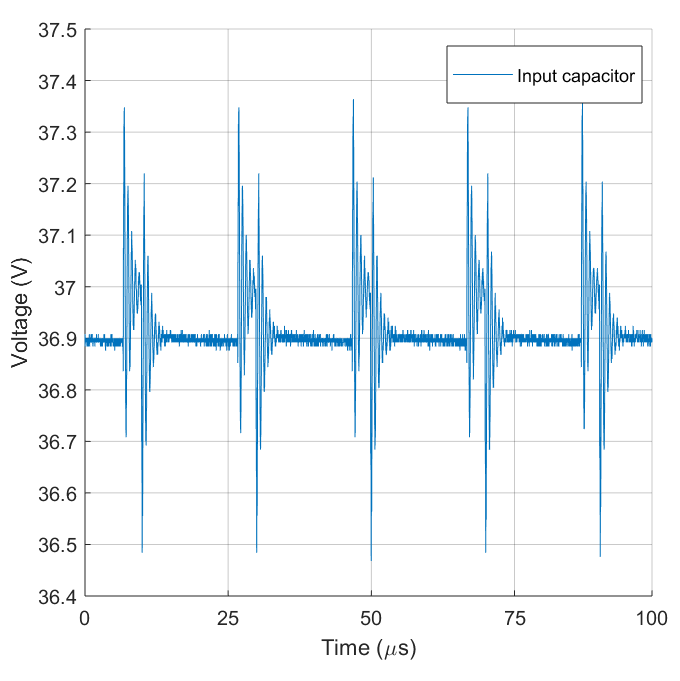
\includegraphics[width=0.65\textwidth]{../Pictures/P1/Test/Openloopinputcapacitor}
		\caption{Open loop test: Input capacitor.}
		\label{Openlooptestinputcapacitor}
	\end{center}	
\end{figure}

\begin{figure}[H]
	\begin{center}
		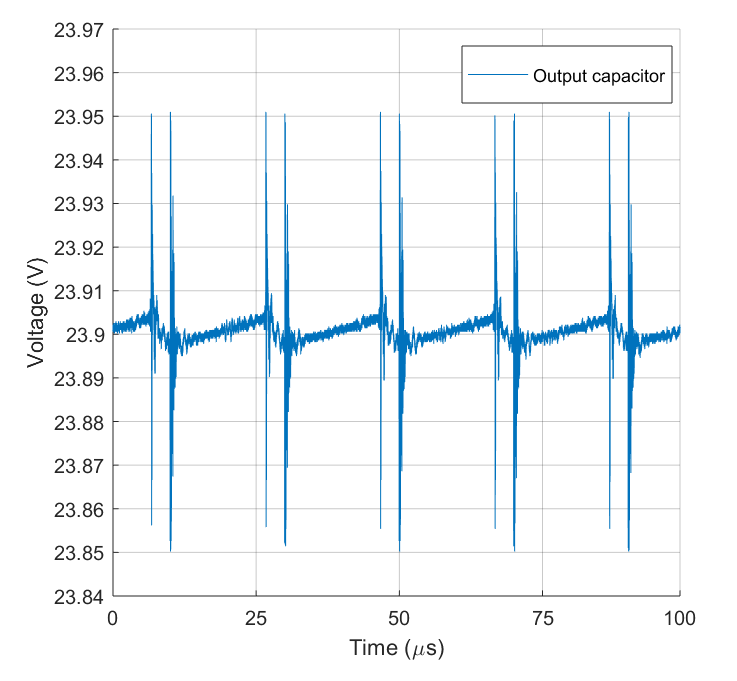
\includegraphics[width=0.65\textwidth]{../Pictures/P1/Test/Openloopoutputcapacitor}
		\caption{Open loop test: Output capacitor.}
		\label{Openlooptestoutputtcapacitor}
	\end{center}	
\end{figure}

\begin{figure}[H]
	\begin{center}
		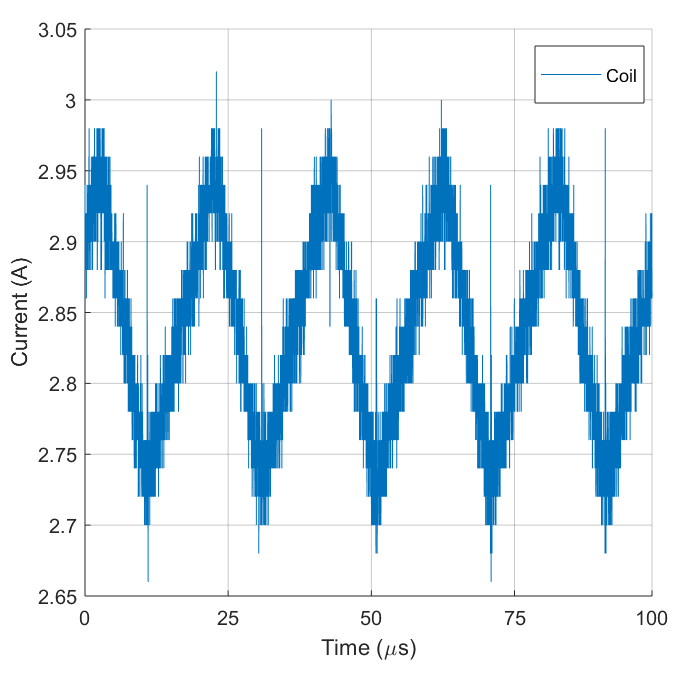
\includegraphics[width=0.65\textwidth]{../Pictures/P1/Test/Openloopinductor}
		\caption{Open loop test: Inductor ripple.}
		\label{Openlooptestinductor}
	\end{center}	
\end{figure}